\documentclass[tikz,border=10pt]{standalone}
\begin{document}
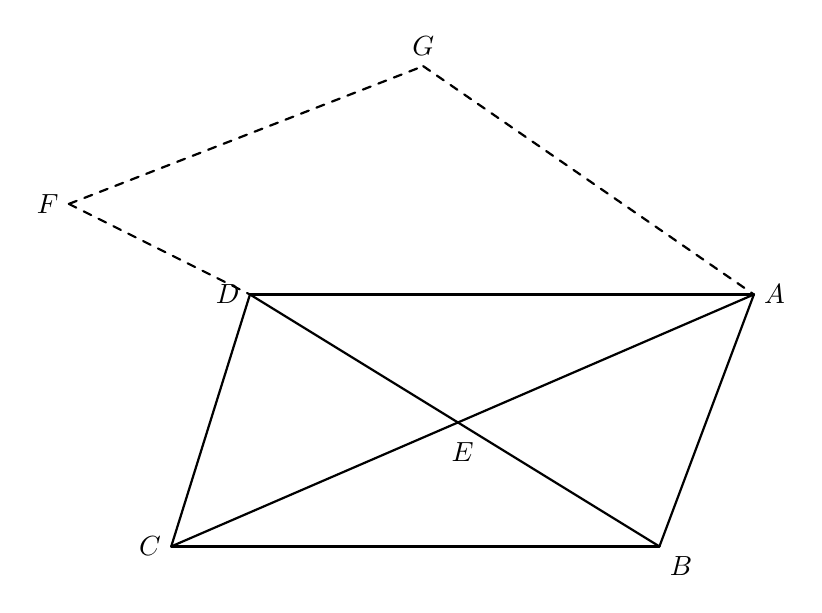
\begin{tikzpicture}[line cap=round,line join=round,thick]

\coordinate (C) at (0,0);
\coordinate (B) at (6.2,0);
\coordinate (D) at (1.0,3.2);
\coordinate (A) at (7.4,3.2);
\coordinate (E) at (3.7,1.45);
\coordinate (F) at (-1.3,4.35);
\coordinate (G) at (3.2,6.1);

\draw (D) -- (A);
\draw (C) -- (B);
\draw (C) -- (D);
\draw (B) -- (A);
\draw (D) -- (B);
\draw (C) -- (A);

\draw[dashed] (F) -- (D);
\draw[dashed] (F) -- (G);
\draw[dashed] (G) -- (A);

\node[left] at (C) {$C$};
\node[below right] at (B) {$B$};
\node[left] at (D) {$D$};
\node[right] at (A) {$A$};
\node[below] at (E) {$E$};
\node[left] at (F) {$F$};
\node[above] at (G) {$G$};

\end{tikzpicture}
\end{document}
